\section{Problem Set 6}

\subsection{Another Control Method}

We realized last week that our method of control from the previous pset was more continuous than impulsive, so we are flipping problem sets 5 and 6. Last weeks implementation is our continuous control (since we can shrink the time step between burns to be zero and thus have continuous thrust), and this week we implemented impulsive control.

For our impulse control this week, we decided to go with a solution to the HCW equations. Since we know where we want to be (docking to the target) we know we want to drive our RTN position to zero. Therefore, we know where we want to be, and if we know where we are, we can solve the HCW equations to determine the delta v we need to apply.

Since:
\begin{align}
r(t) = \Phi_{rr}r_0 + \Phi_{rv}v_0
\end{align}

We can set the final position to be zero (since we are docking) and rearrange to get
\begin{align}
v_0 = -\Phi_{rv}^{-1}\Phi_{rr}r
\end{align}

Thus, we can solve what the velocity needs to be after the maneuver, and if we know the starting RTN velocity we can calculate the delta v of the maneuver.

This methodology has several advantages. First, it can always take the position of the spacecraft and generate a necessary delta v to reach the target at a specified time frame. By decreasing the time frame, one can decrease delta v costs. However, it leaves the time frames (in terms of when to burn as well as how long the transfer will take) up to the user, which means there could be suboptimal solutions requested.

Below is the results of this methodology in our simulator. As you can see, from an arbitrary RTN starting state with arbitrary position and velocity, the solver is able to calculate the necessary trajectory and execute it to intercept the target spacecraft.


\begin{figure}[H]
    \centering
    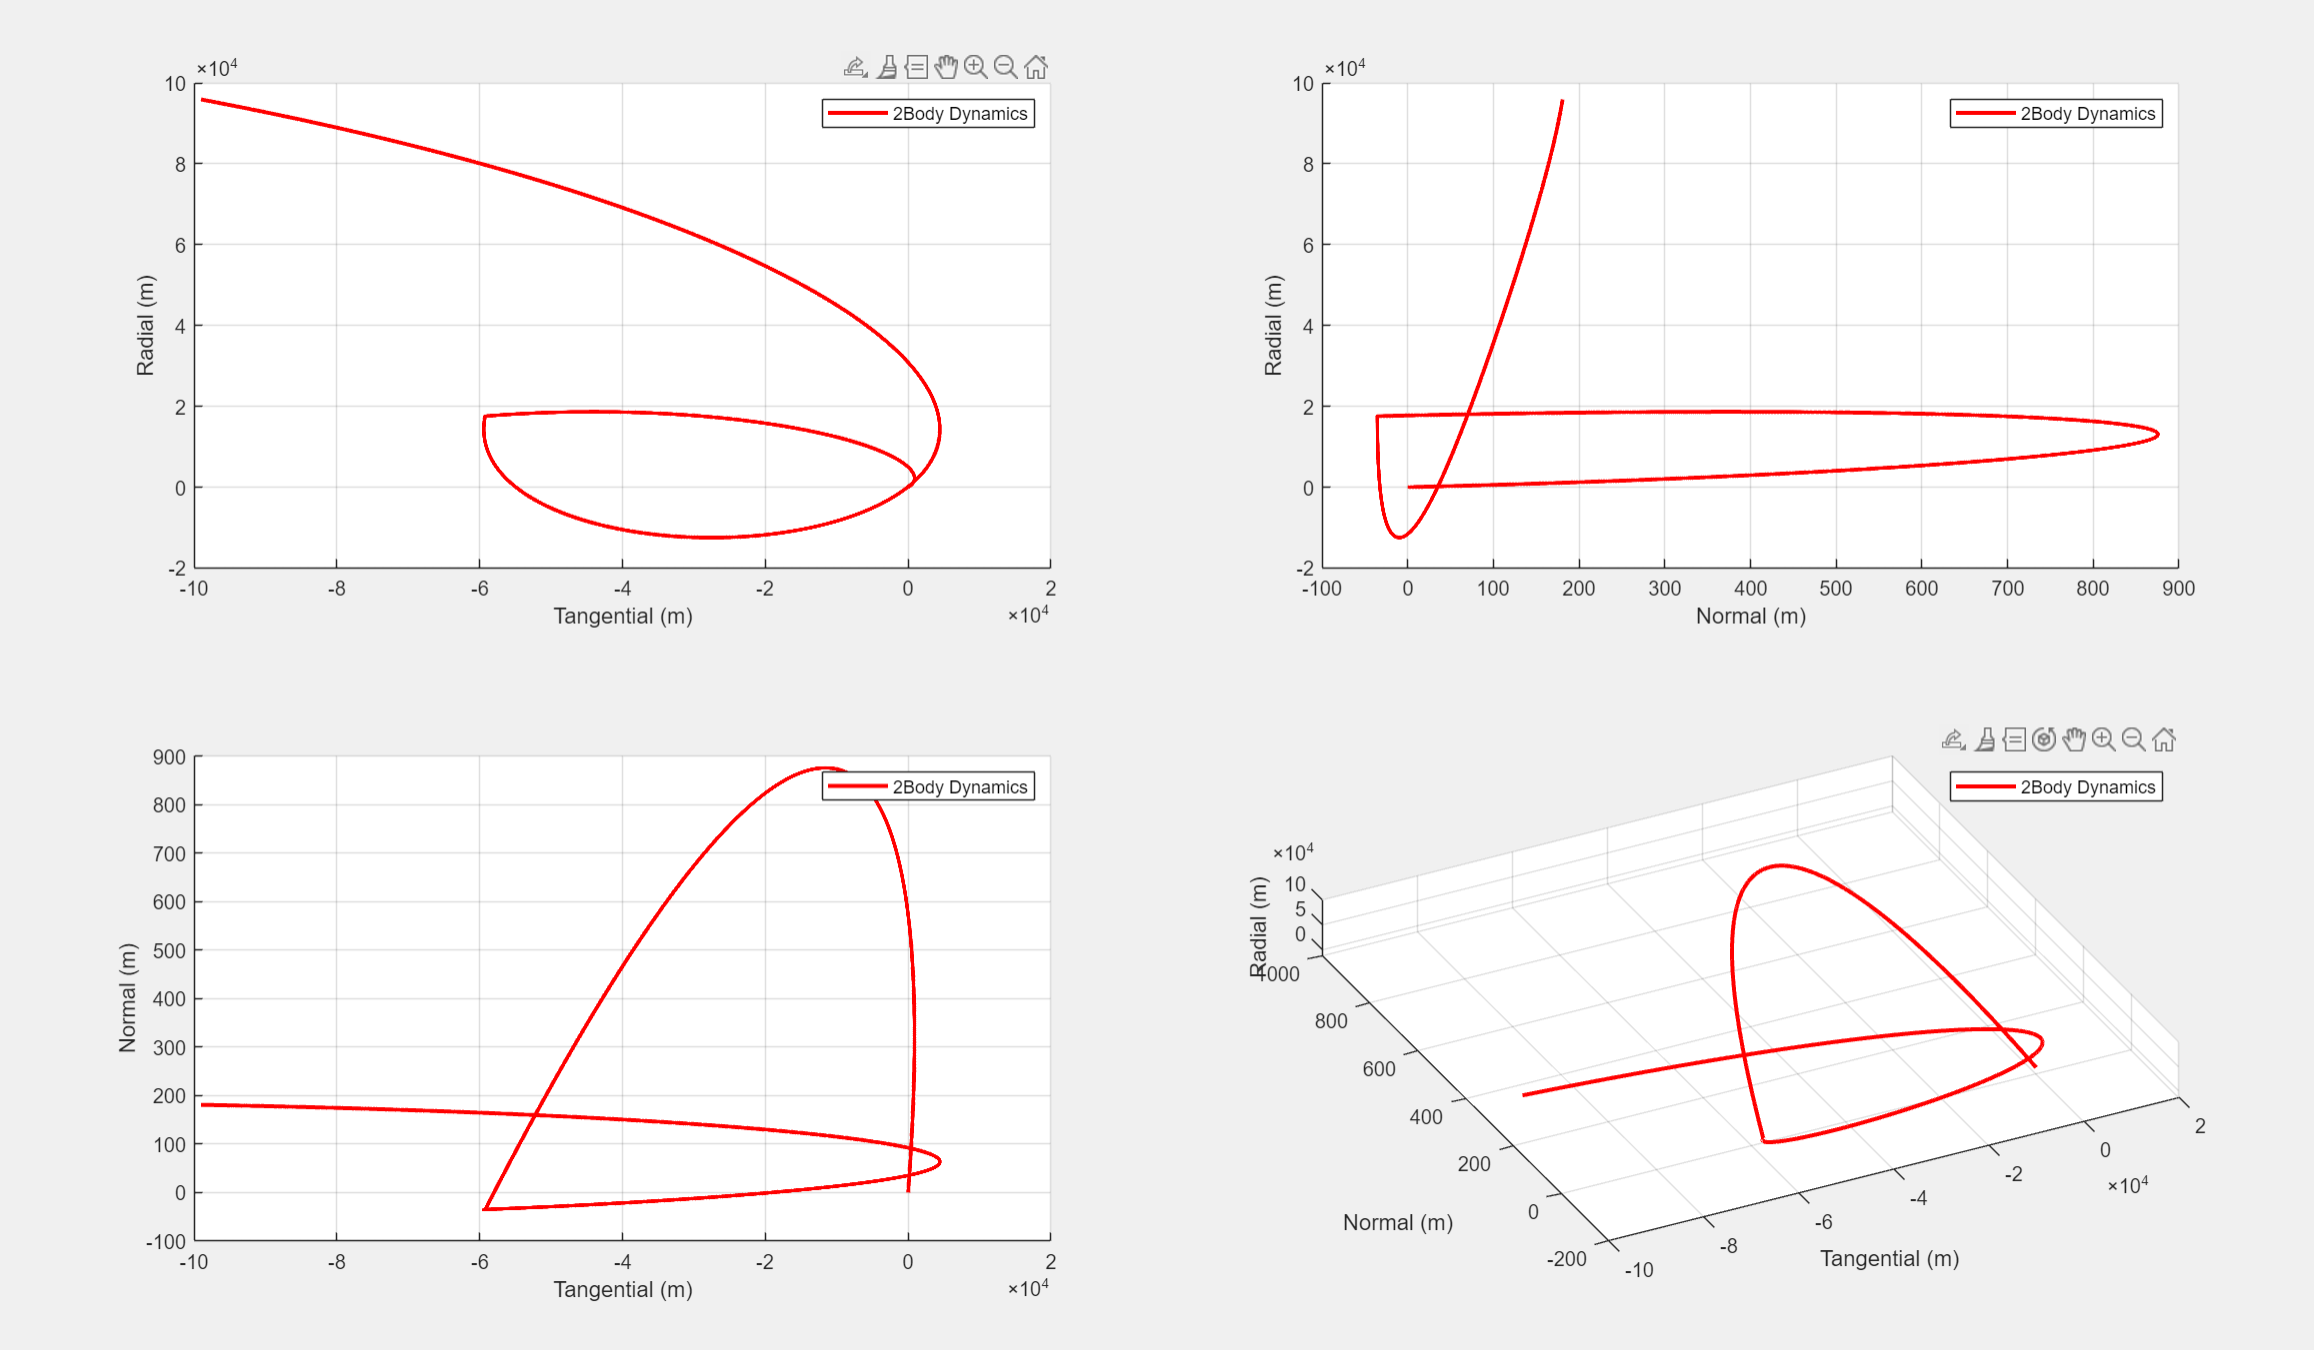
\includegraphics[width=0.7\textwidth]{PS6/Figures/trajectory.png}
    \caption{RTN Trajectory}
    \label{fig:hcw_velocity}
\end{figure}

\begin{figure}[H]
    \centering
    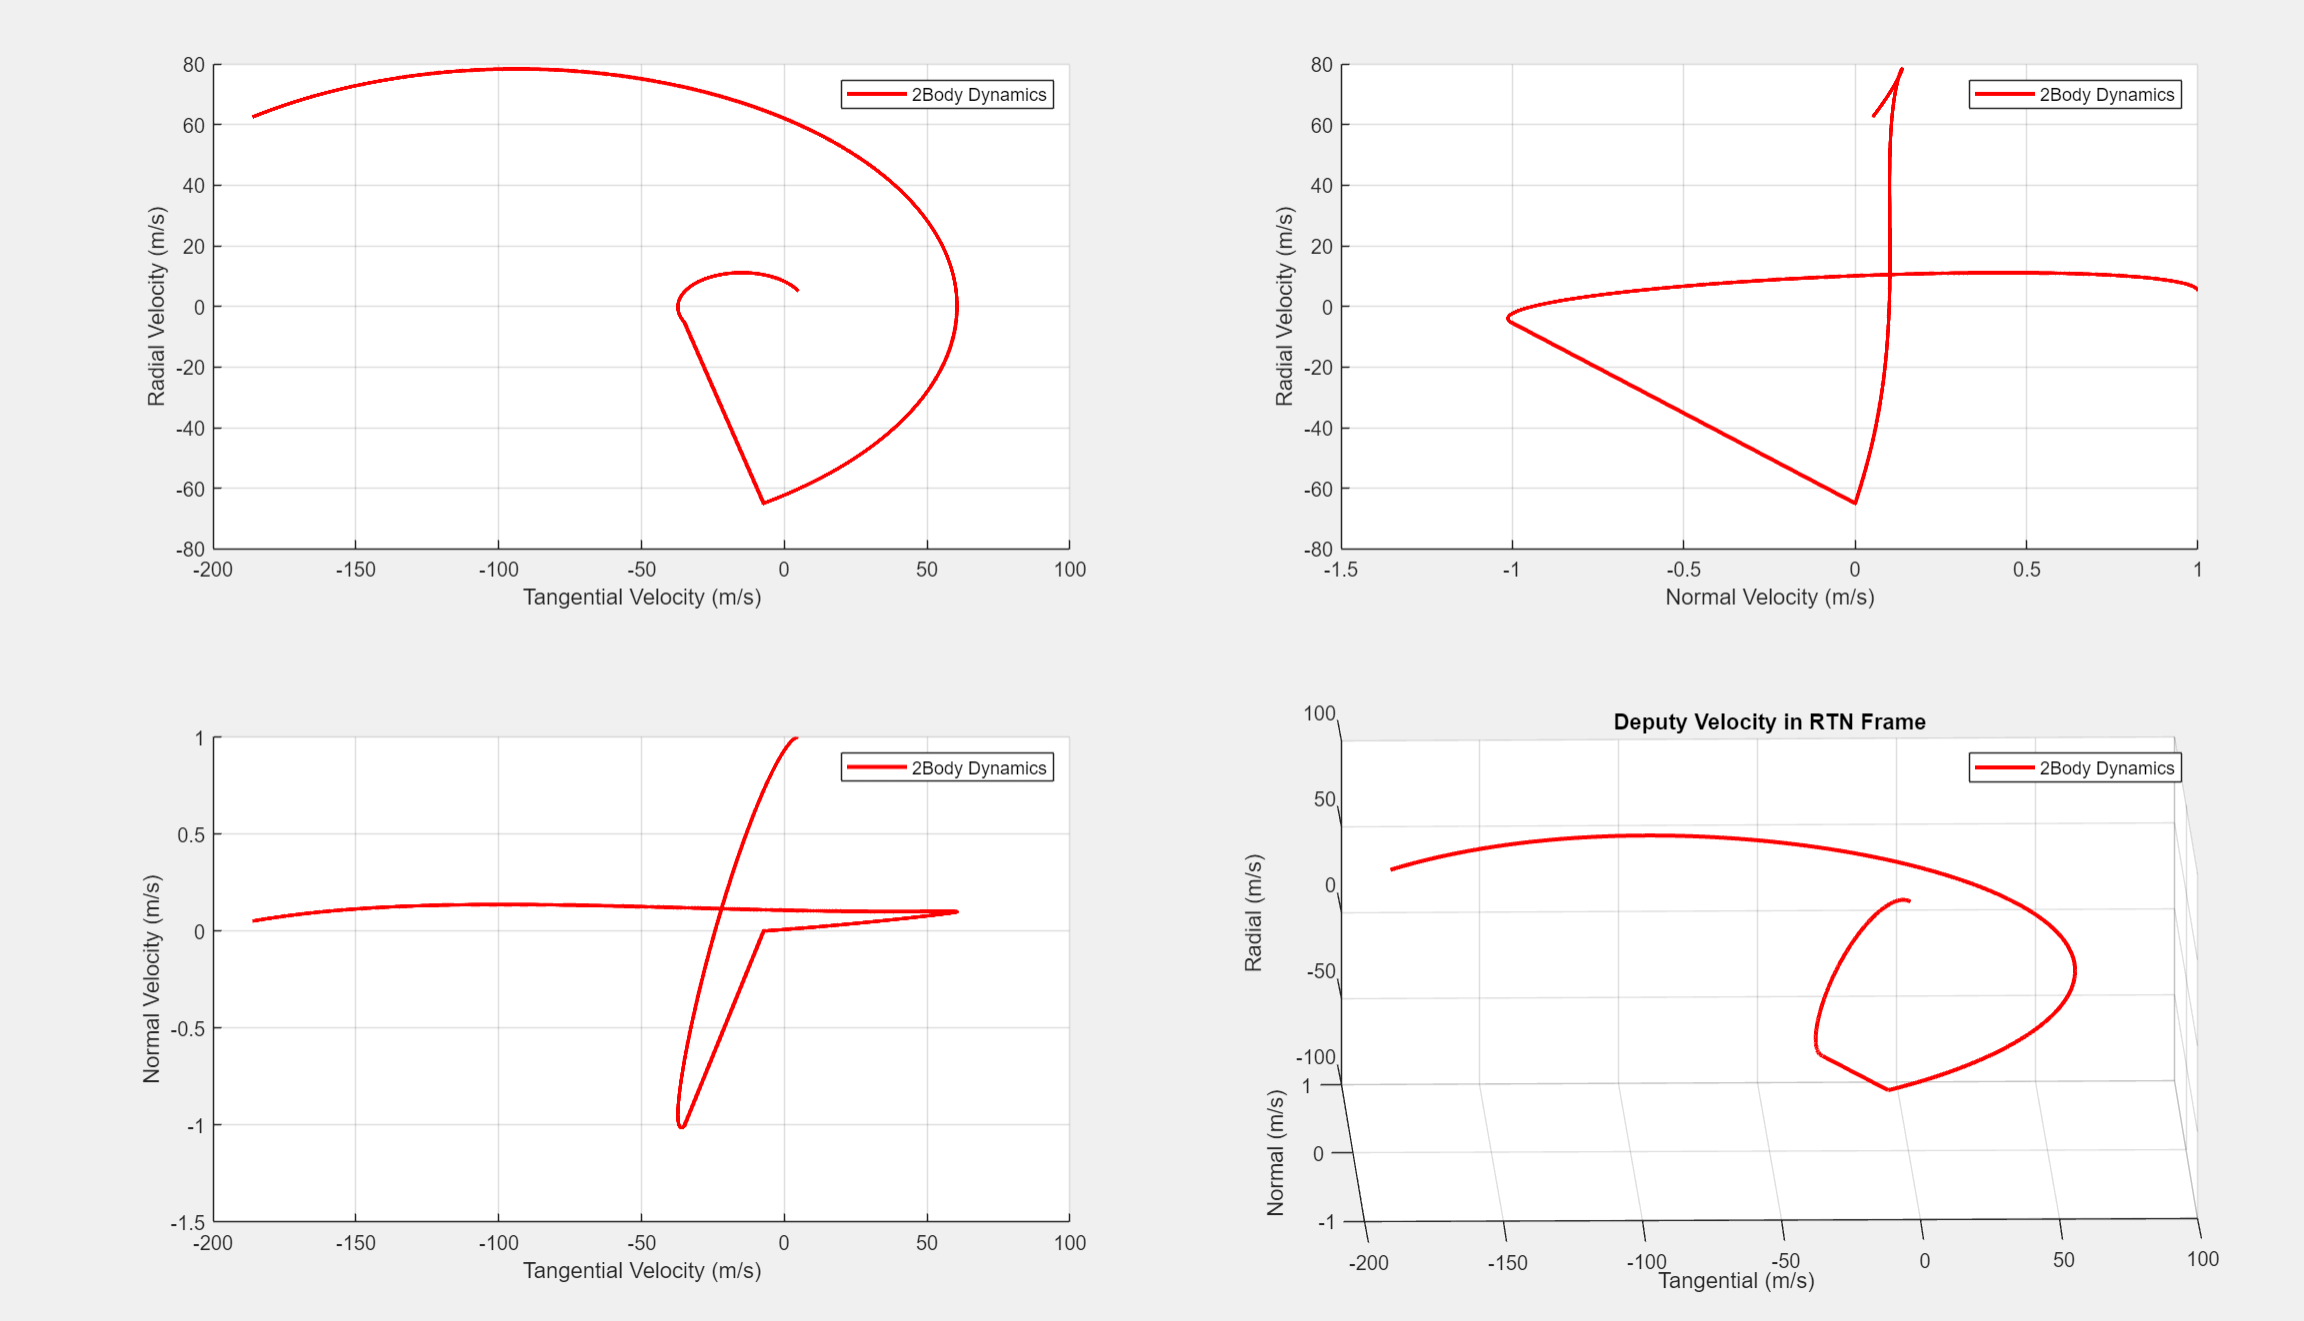
\includegraphics[width=0.7\textwidth]{PS6/Figures/velocity.png}
    \caption{RTN Velocity}
    \label{fig:hcw_velocity}
\end{figure}

We will not include a delta v plot over time for this problem, since it is rather simple - a single increase in delta v at one point in time.

Beyond the issues discussed above, this methodology has additional problems. First, it only works well in circular orbits due to it's reliance on HCW.

Our ground-truth simulation uses two-body dynamics for both spacecraft, implementing the impulsive maneuver as an instantaneous change in velocity at the calculated burn time. This implementation assumes perfect knowledge of the state vectors and perfect execution of the burn. In a real-world scenario, navigation errors and thruster imperfections would cause deviations from the planned trajectory.

This method also assumes small relative distances between spacecraft since the HCW equations are linearized around the reference orbit. For larger separations, the linear approximation breaks down and leads to targeting errors.

Unlike our continuous control approach from last week which required multiple small corrections, this impulsive method requires just a single, well-timed burn to achieve the desired rendezvous. While our continuous approach provides more robustness against disturbances and modeling errors by constantly adjusting the trajectory, this impulsive method is significantly more fuel-efficient for scenarios where the dynamics are well-known and external perturbations are minimal.

The single impulsive maneuver calculated by our algorithm approaches the theoretical minimum delta-v for a direct rendezvous transfer in circular orbits using HCW dynamics, making it particularly attractive for spacecraft with limited propellant budgets. However, this efficiency comes at the cost of flexibility and robustness that continuous control methods provide.